\documentclass[svgnames]{beamer}
\usetheme{Dresden}
\usecolortheme{beaver}
\usepackage{textcomp}
\usepackage{color}
\usepackage{colortbl}
\usepackage{pbox}
\setbeamerfont{page number in head/foot}{size=\large}
\setbeamertemplate{footline}[frame number]
\title{An experimental study of the learnability of congestion control}
\author{Anirudh~Sivaraman, Keith~Winstein, Pratiksha~Thaker, Hari~Balakrishnan}
\institute{MIT CSAIL\vspace{\baselineskip}\\\textcolor{DarkBlue}{http://web.mit.edu/remy/learnability}
}
%\\\textcolor{DarkBlue}{http://web.mit.edu/anirudh/www/sdn-data-plane.html}}
%\date{}

\begin{document}

\begin{frame}

\titlepage

\end{frame}

\begin{Large}
\begin{frame}
\frametitle{Congestion-control protocols today}
\begin{itemize}
\item<2-> Implicitly assume certain network conditions
\item<3-> Implicit performance goals
\end{itemize}
\end{frame}

\begin{frame}
\frametitle{But, assumptions are always wrong}
What if
\begin{itemize}
\item<2-> Links get much faster? (transatlantic cables, datacenters)
\item<3-> Degree of multiplexing shoots up? (incast)
%\item<3-> Delays get longer: satellite links
\end{itemize}
\end{frame}

\begin{frame}
\frametitle{This talk}
\begin{center}
How easy is it to “learn” a network protocol to achieve a desired goal,
despite an imperfect set of assumptions?
\end{center}
\end{frame}

\begin{frame}
\frametitle{Automating protocol design}
\noindent \only<2>{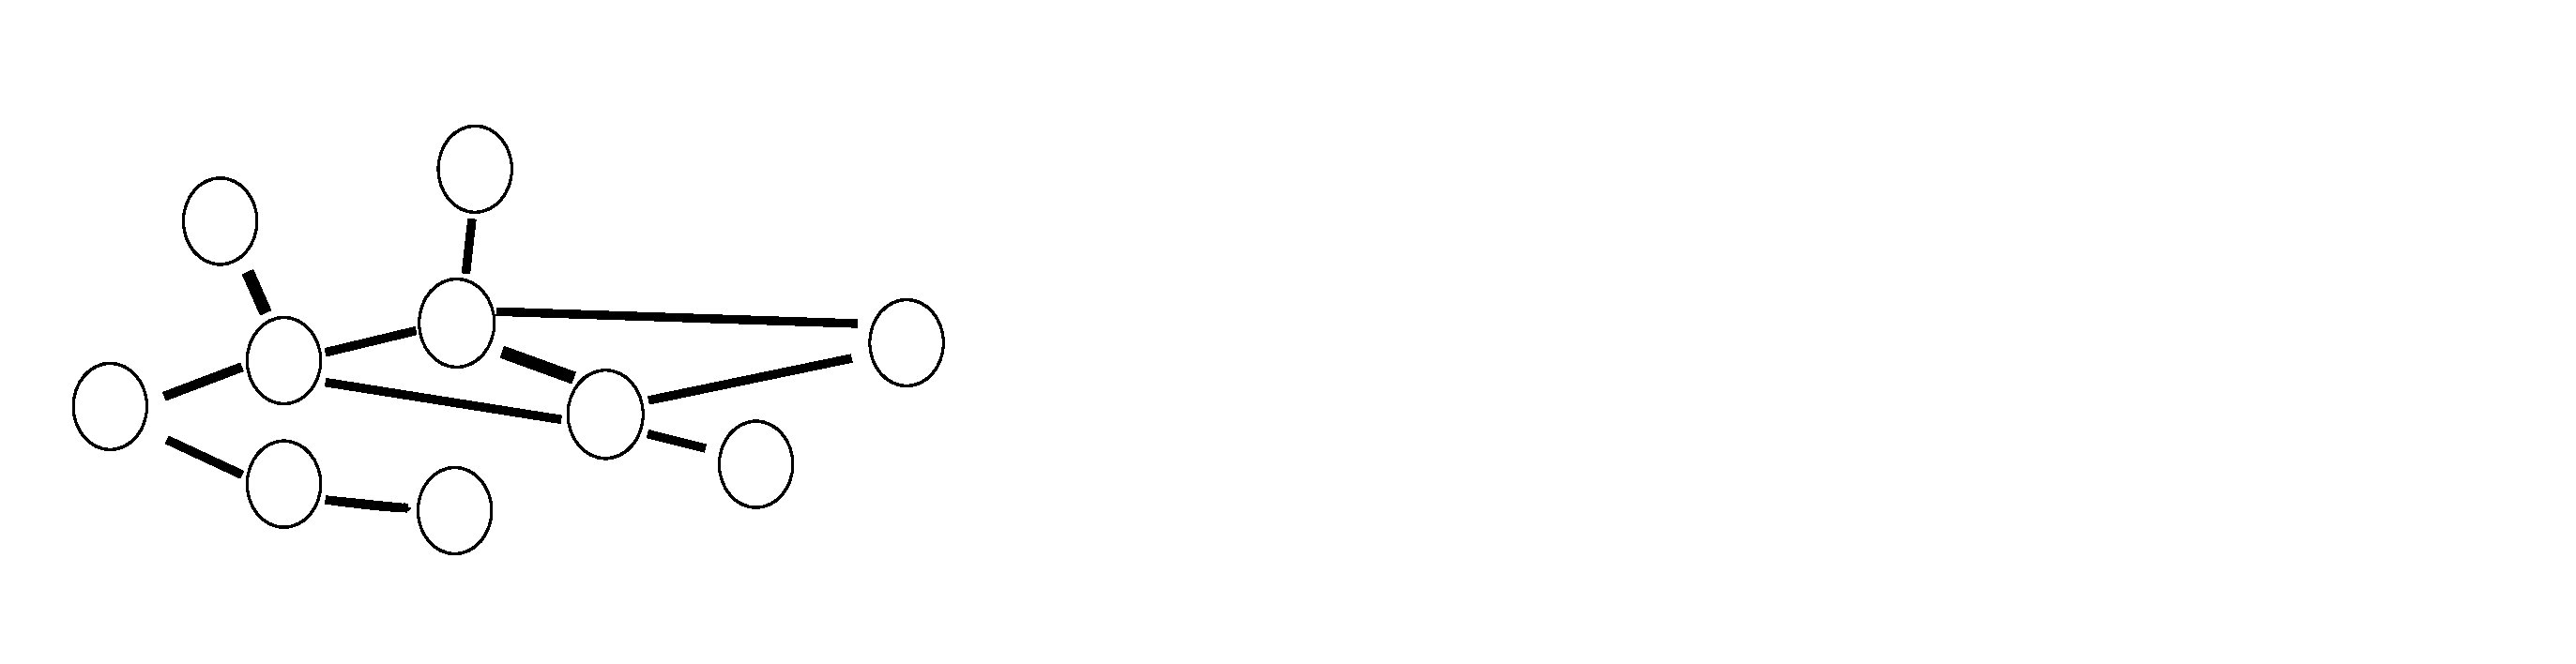
\includegraphics[width=5.5 in]{network-base.pdf}}\only<3>{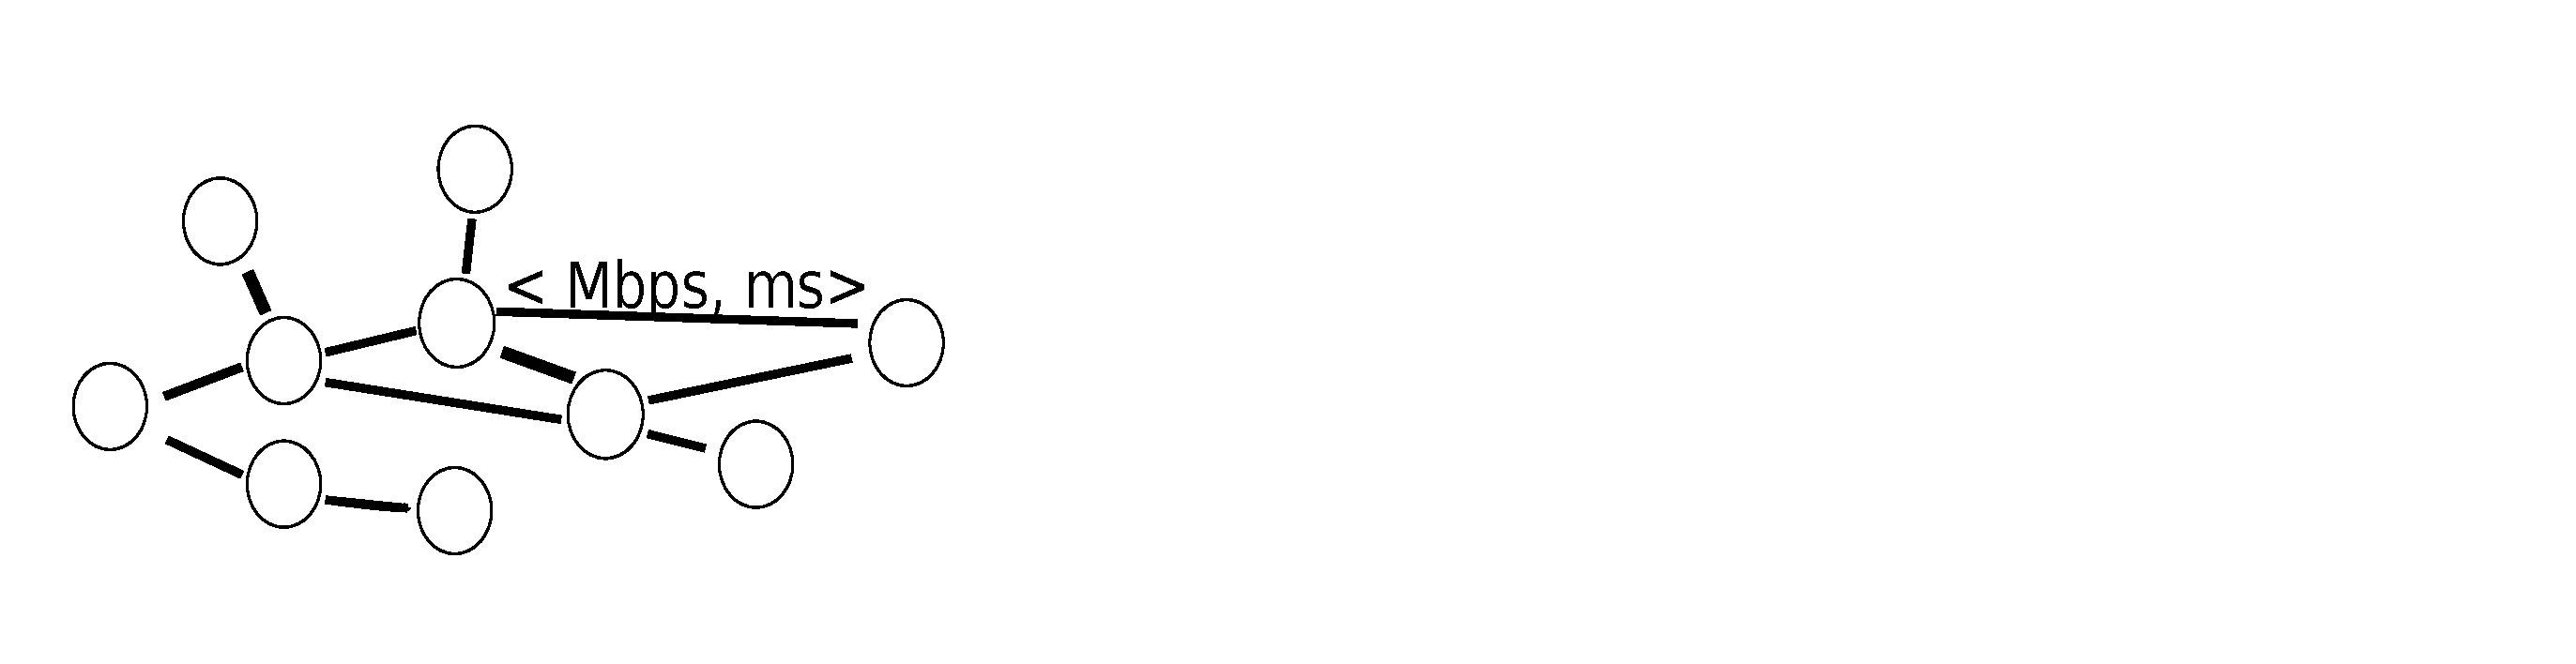
\includegraphics[width=5.5 in]{network-link.pdf}}\only<4>{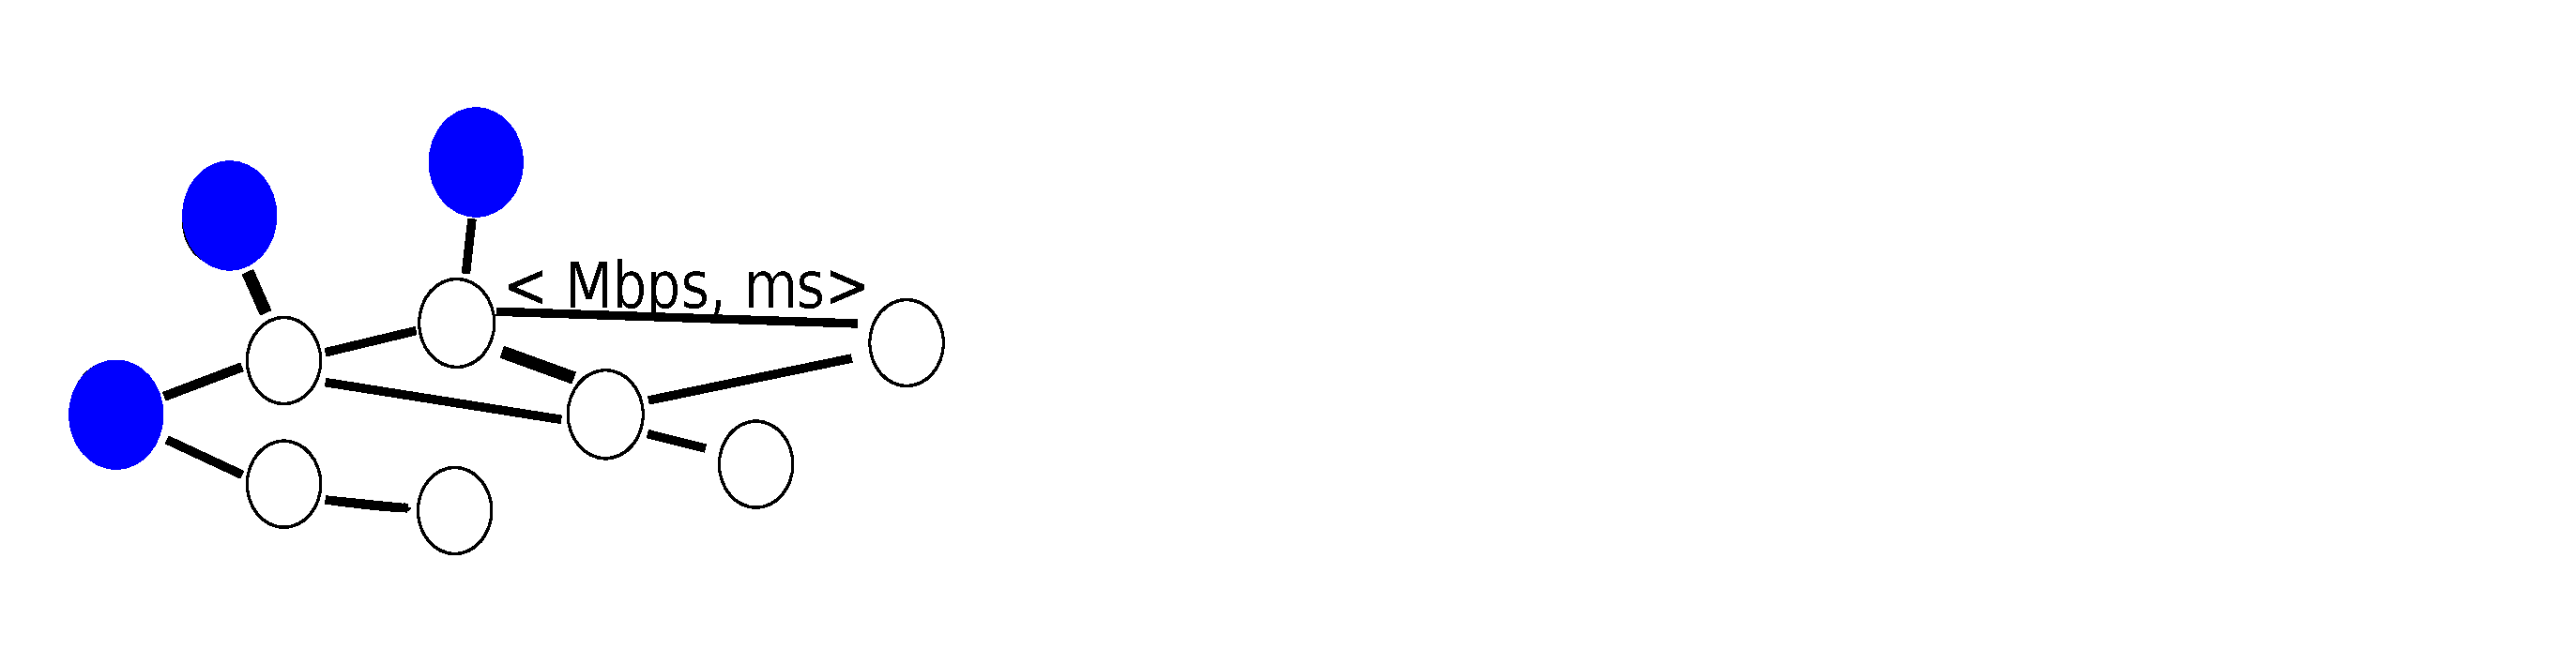
\includegraphics[width=5.5 in]{network-senders.pdf}}\only<5>{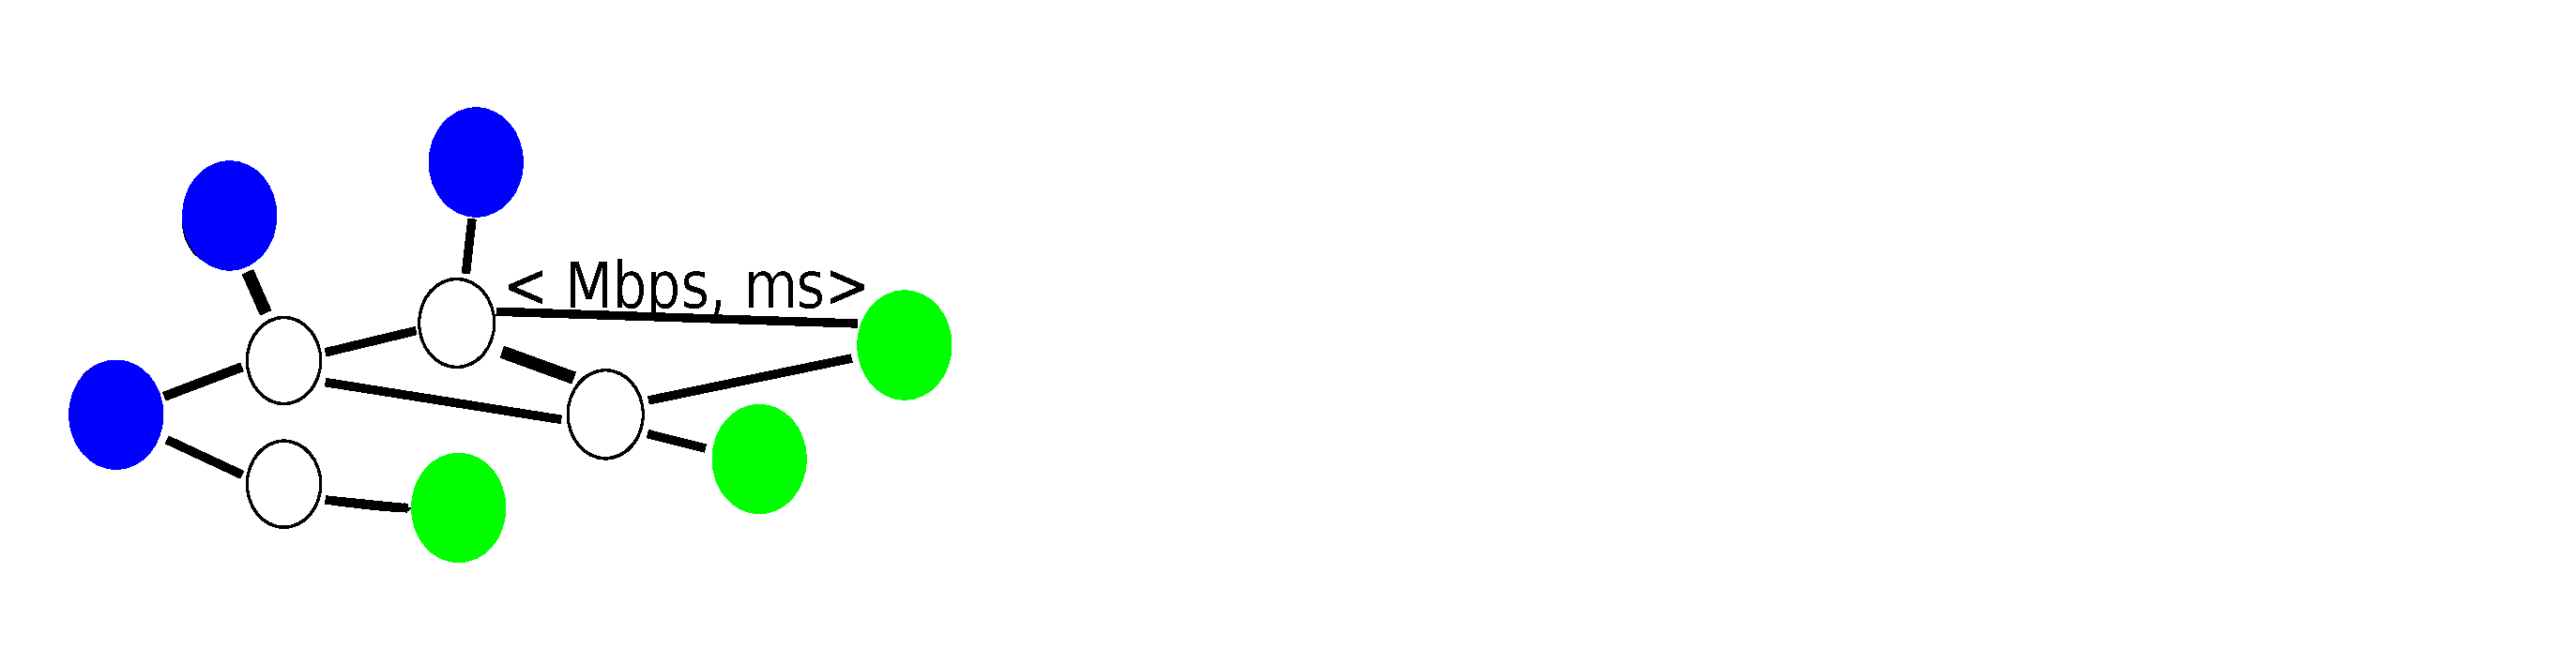
\includegraphics[width=5.5 in]{network-receivers.pdf}}\only<6>{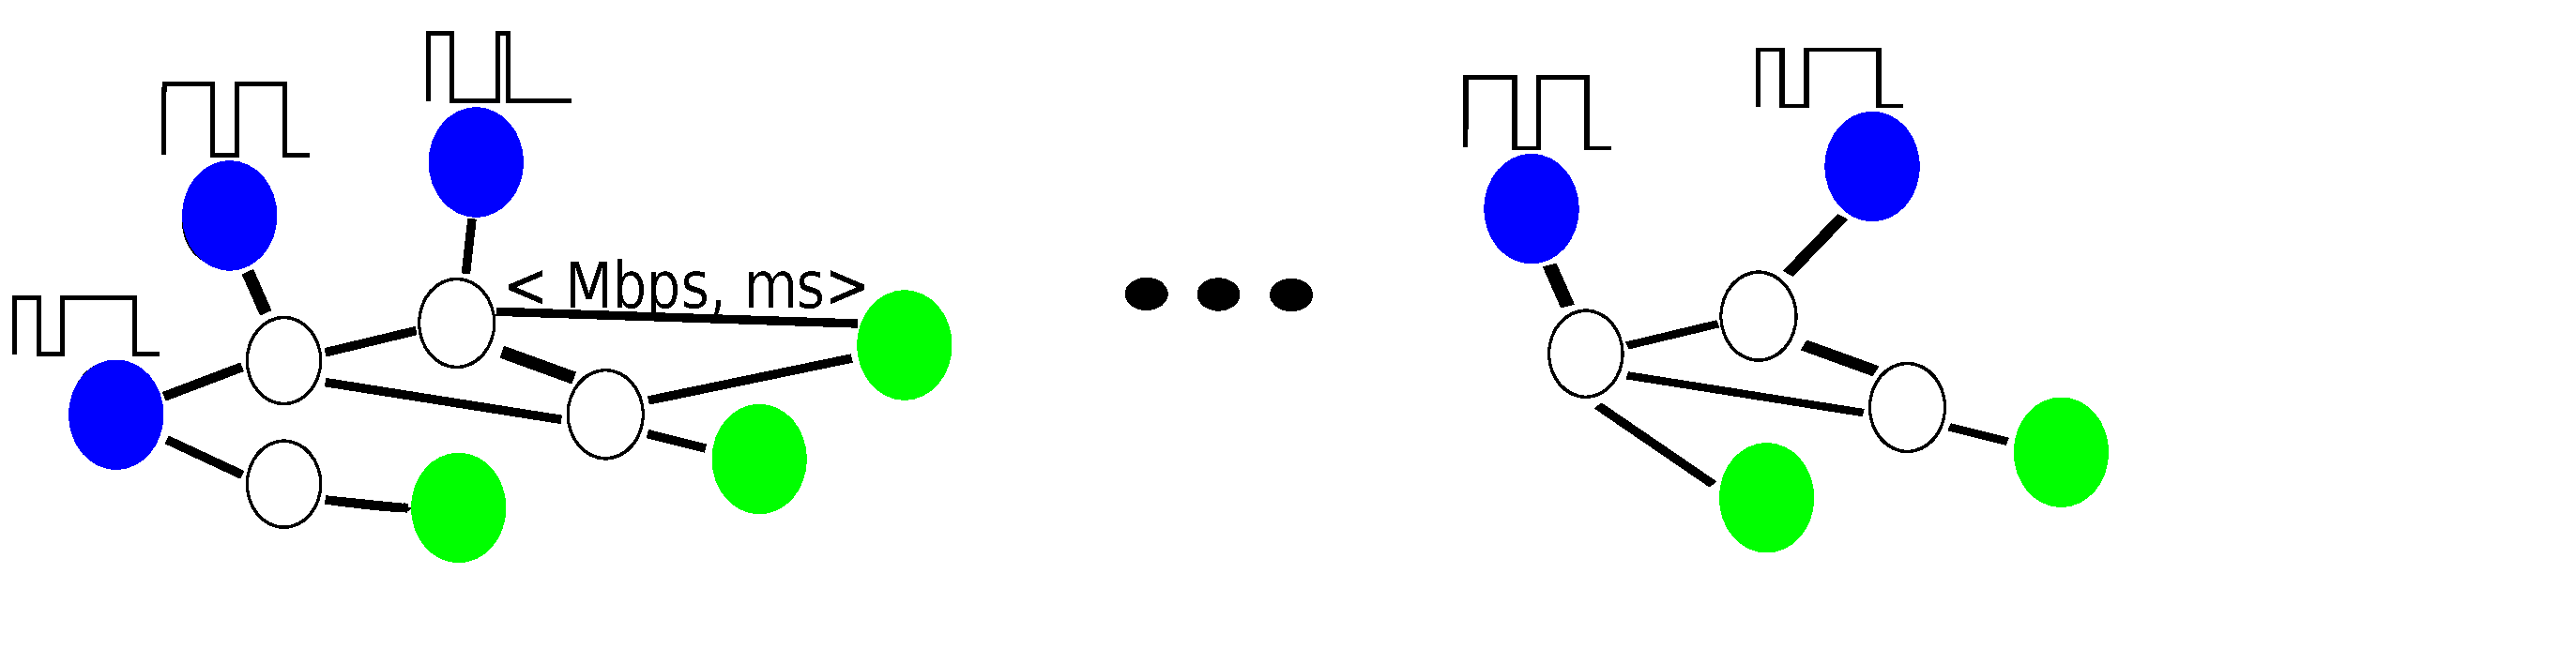
\includegraphics[width=5.5 in]{network-onemore.pdf}}
\end{frame}

\begin{frame}
\frametitle{Automating protocol design}
\noindent \only<1>{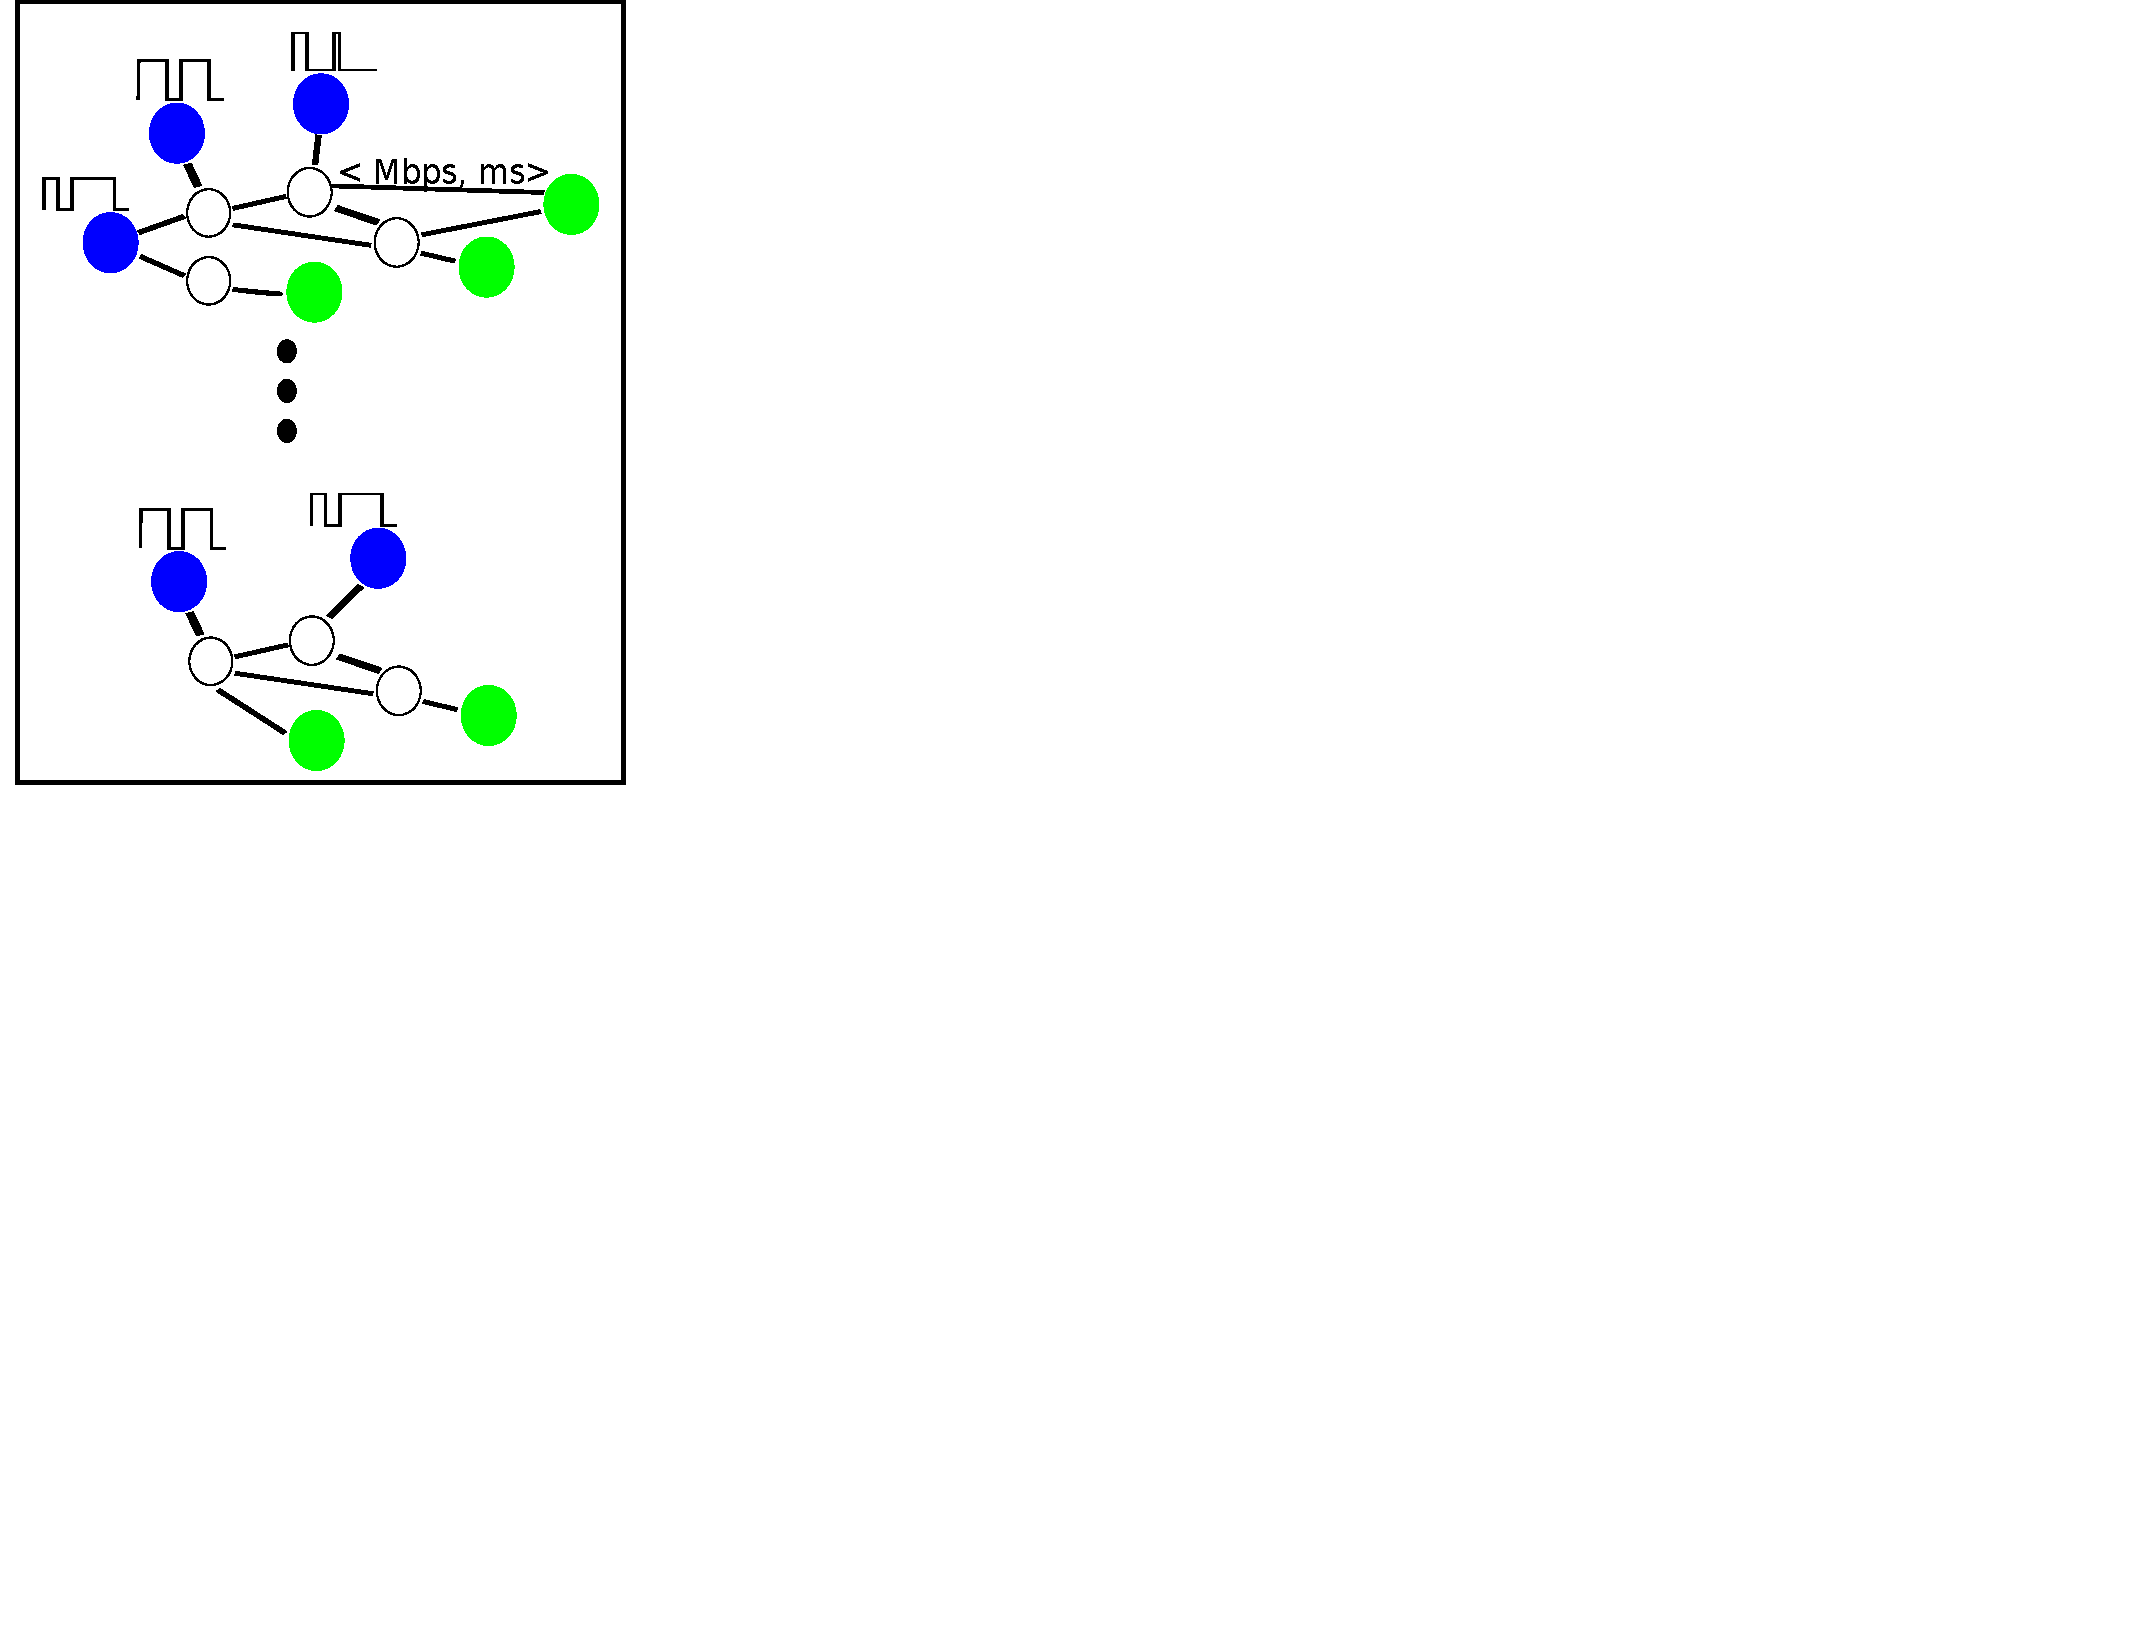
\includegraphics[width=3.5 in]{mechanize-1.pdf}}\only<2>{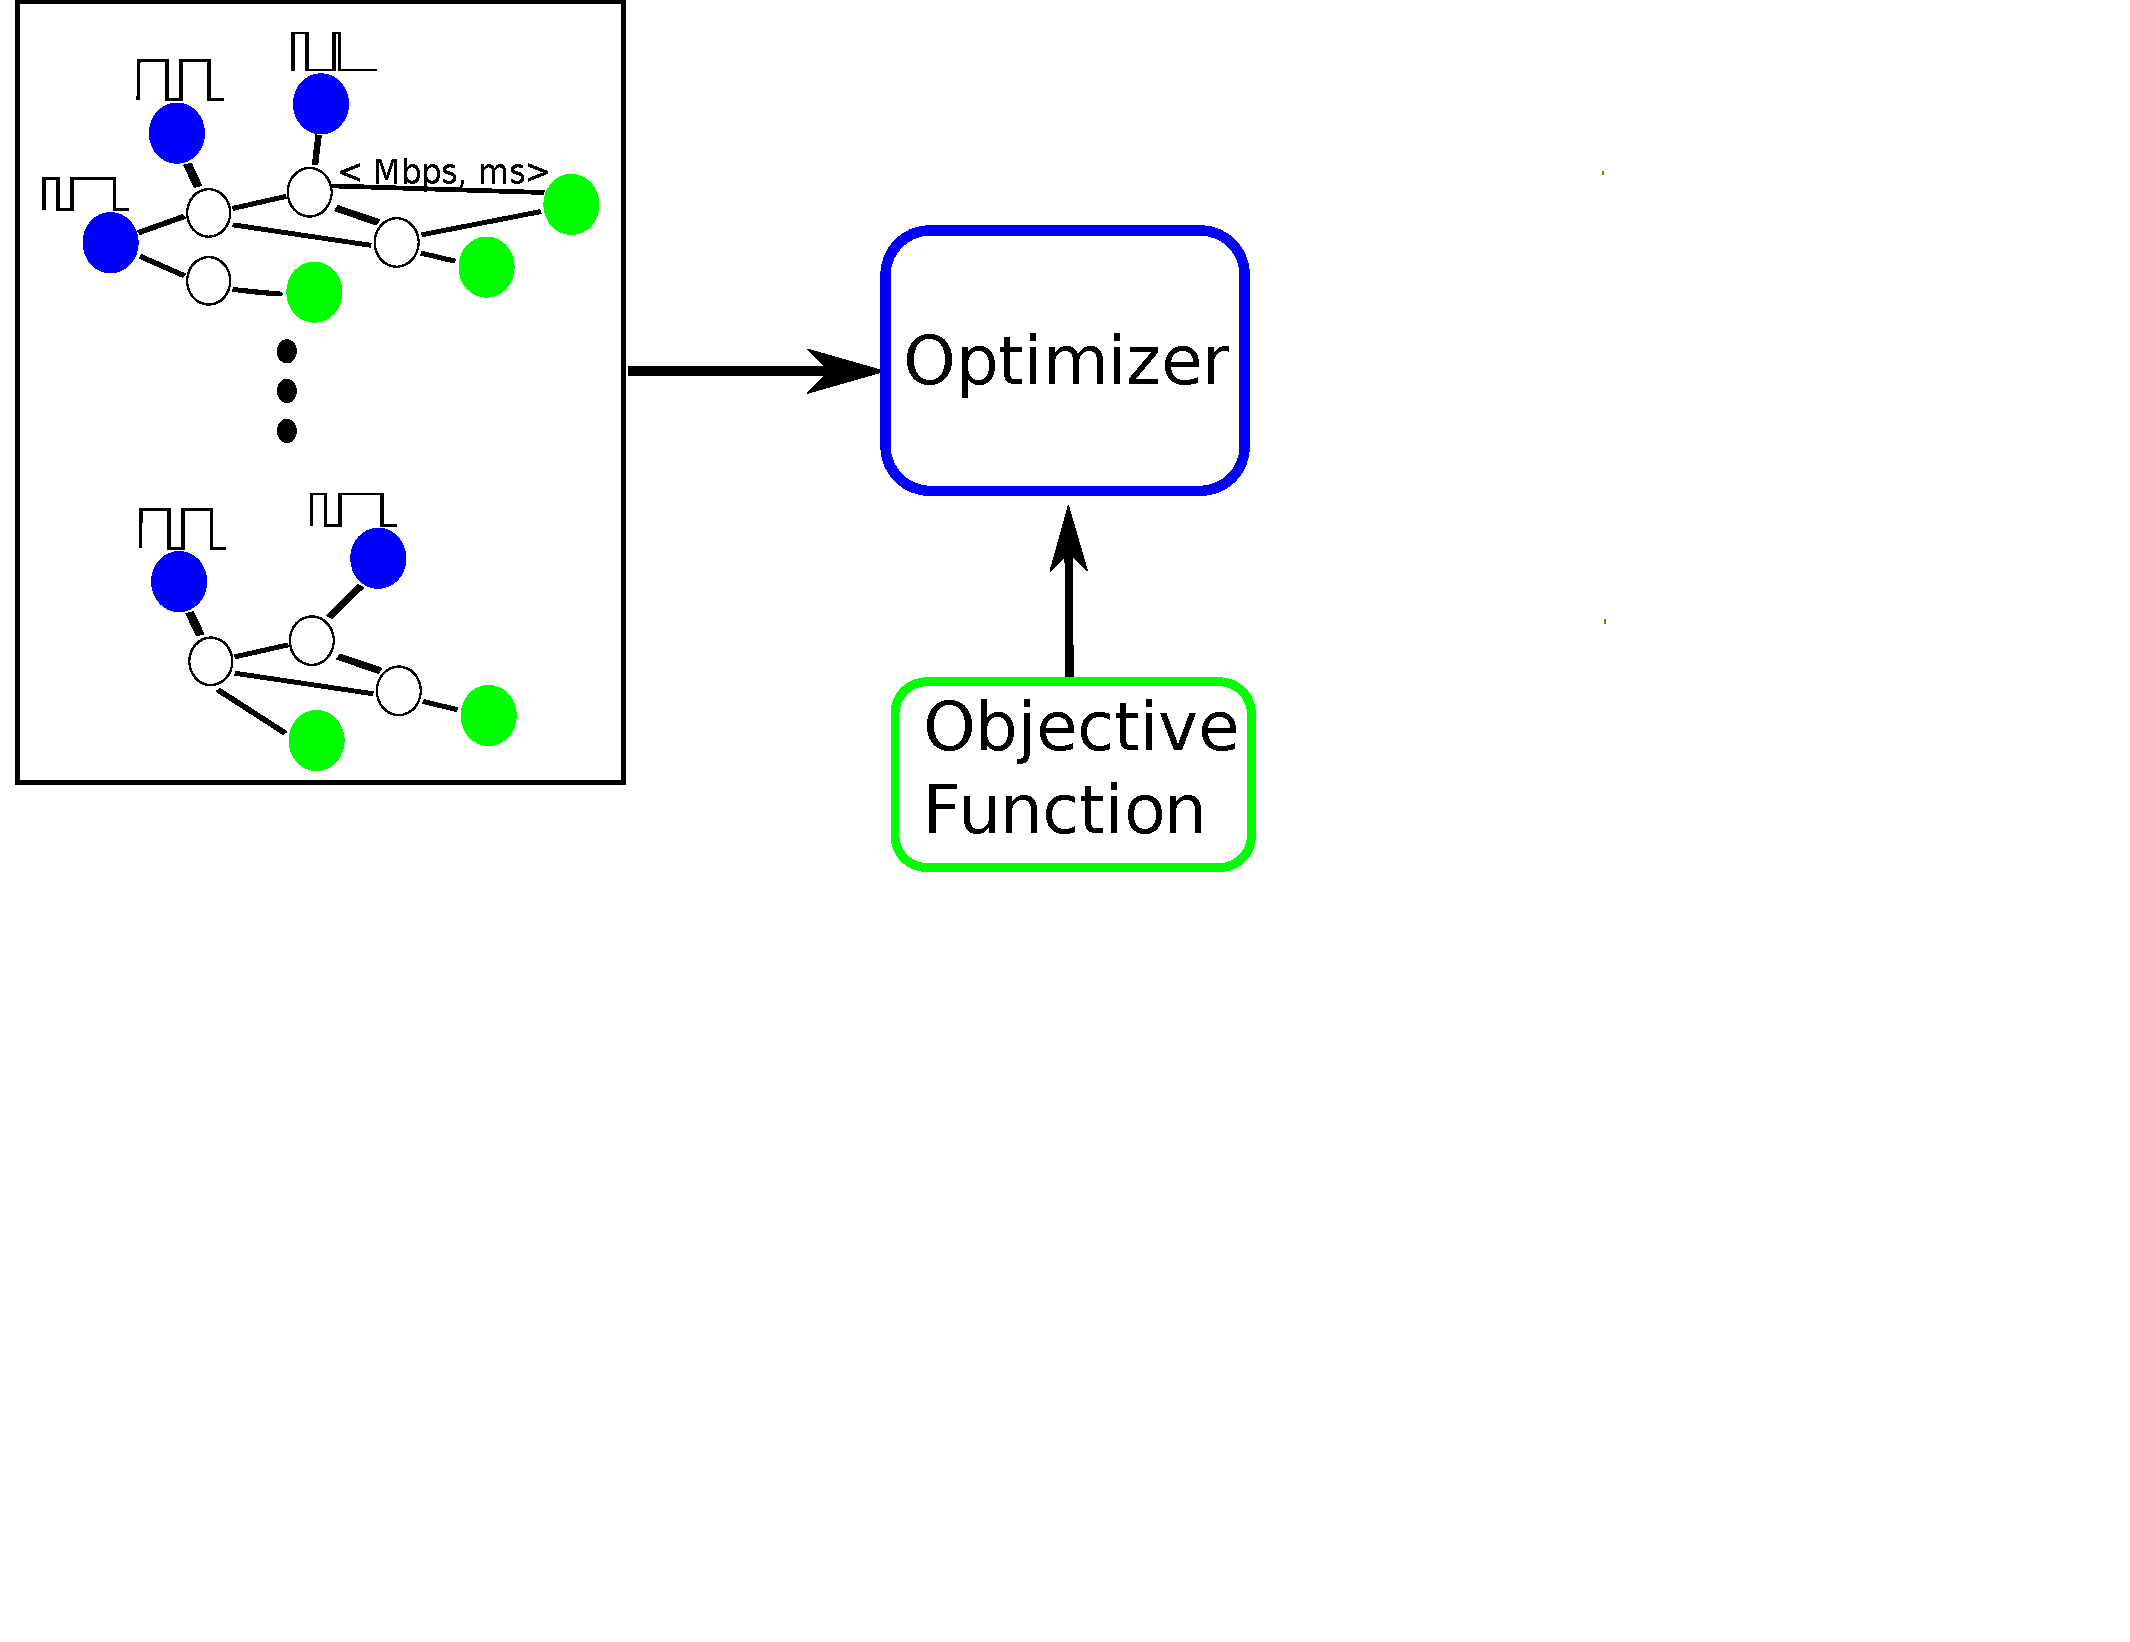
\includegraphics[width=3.5 in]{mechanize-2.pdf}}\only<3>{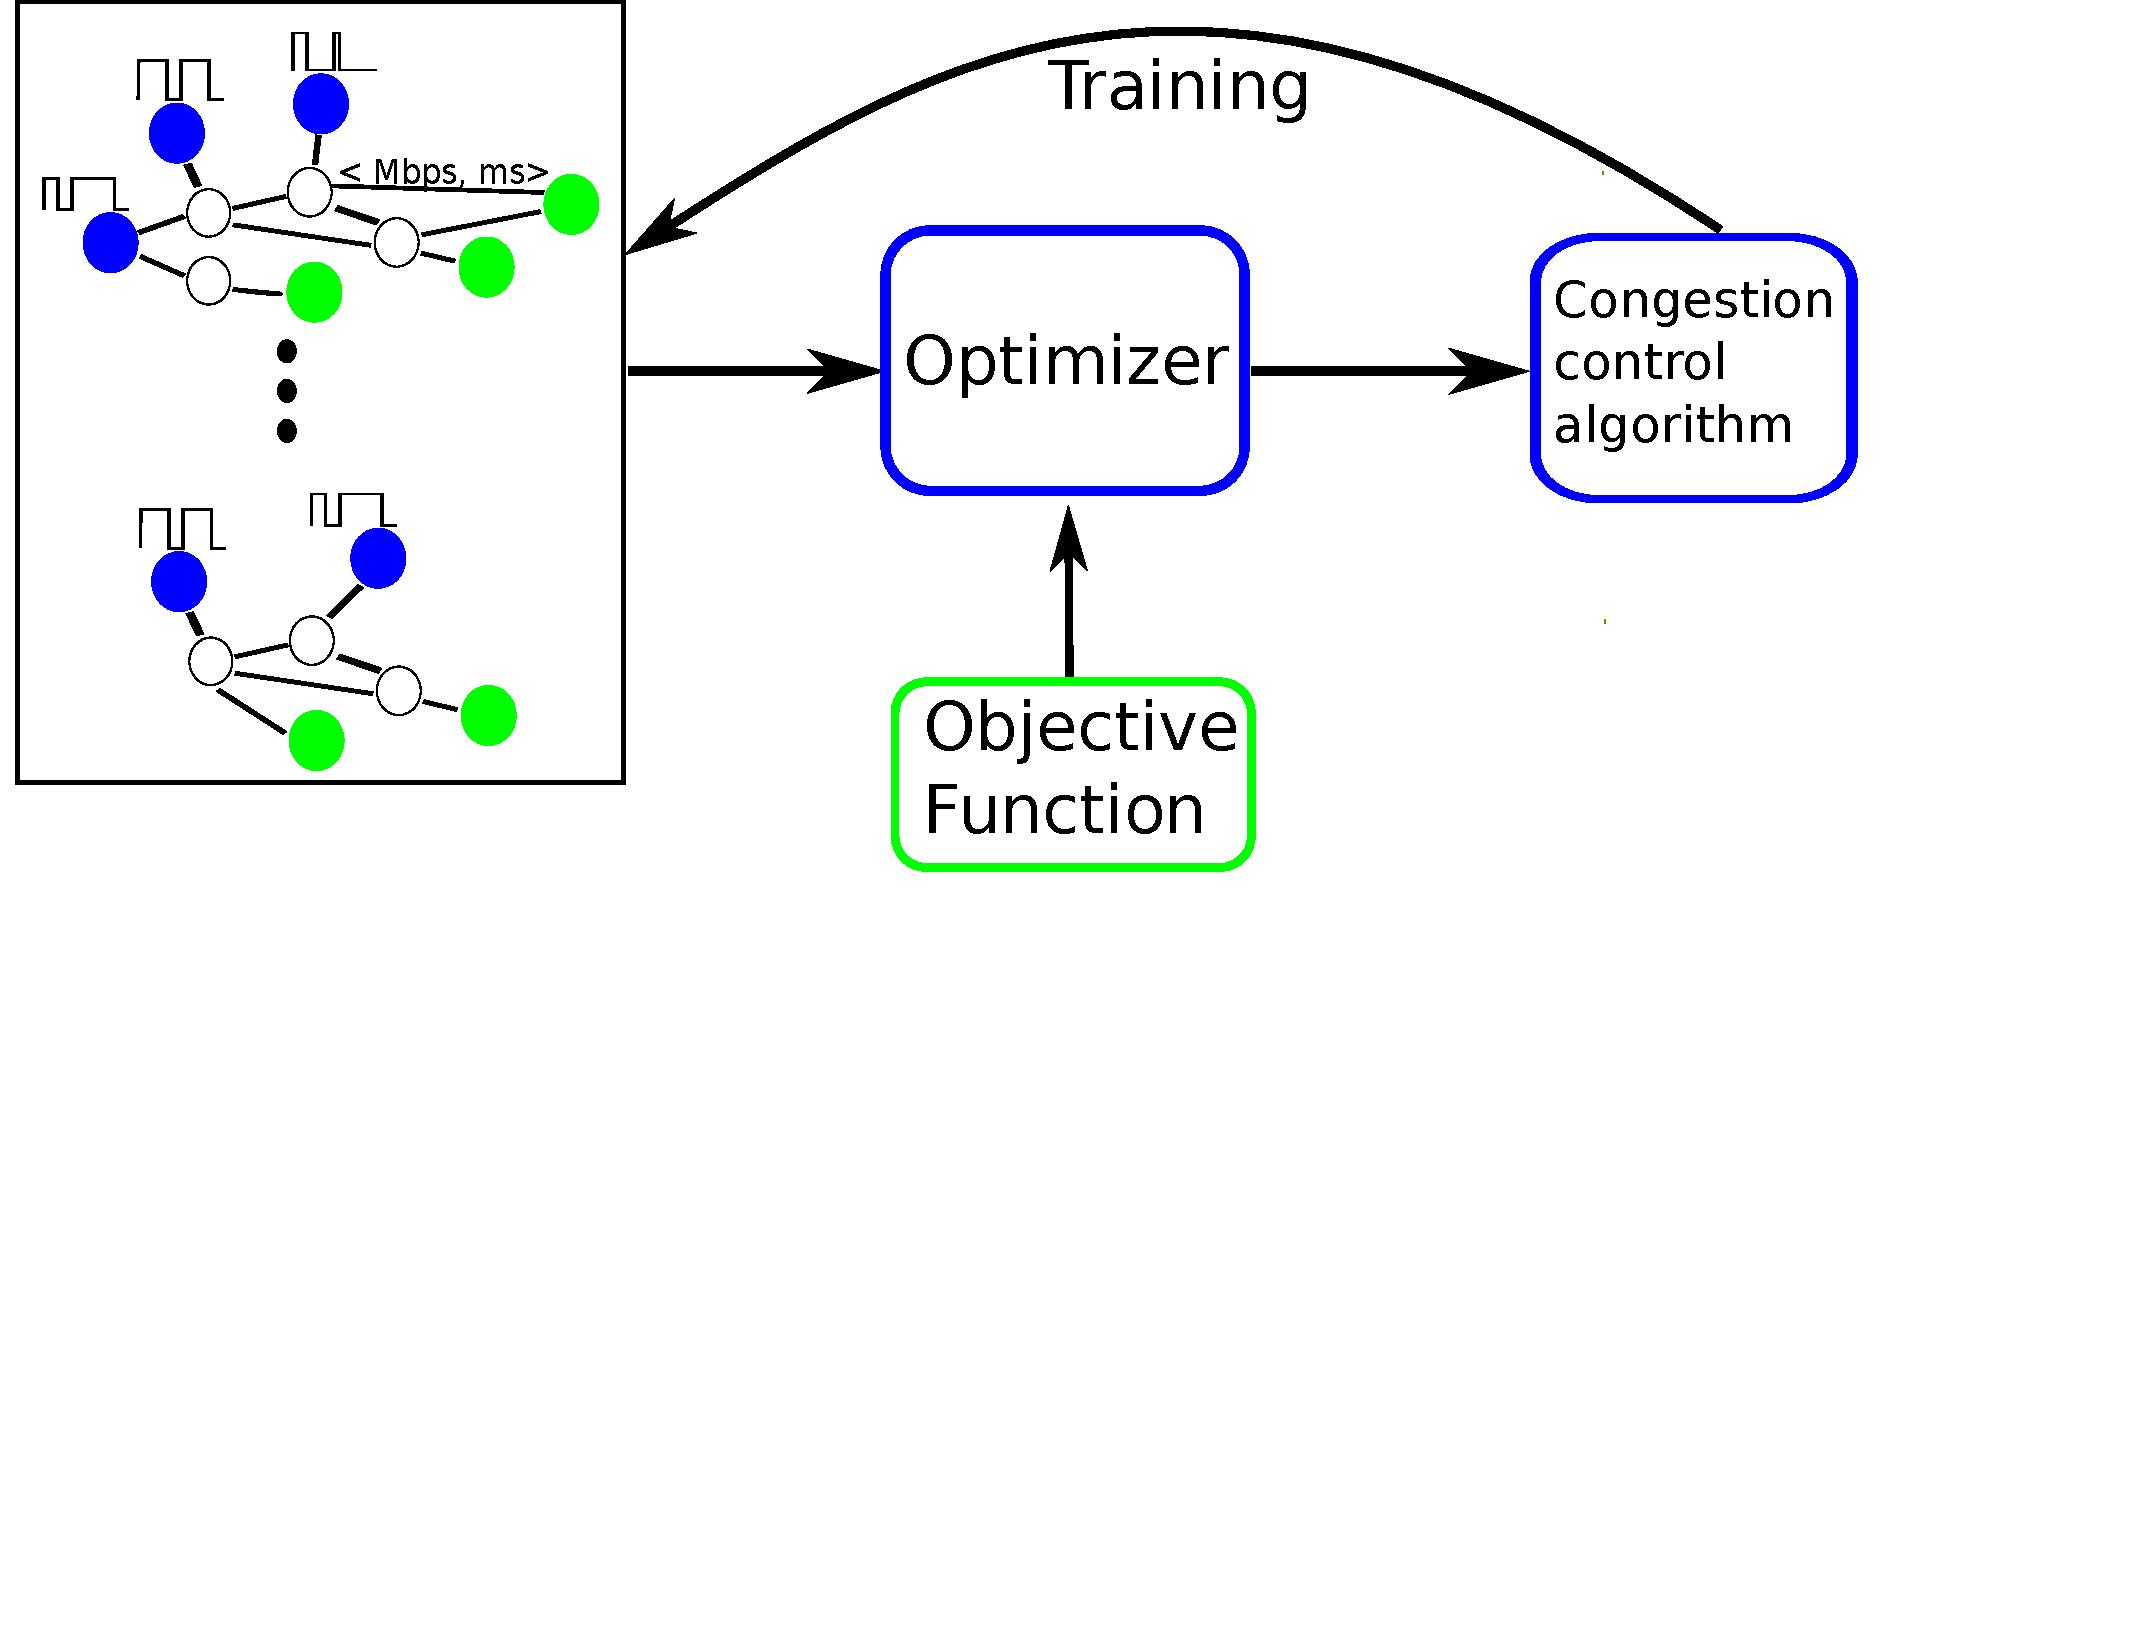
\includegraphics[width=3.5 in]{mechanize-3.pdf}}\only<4>{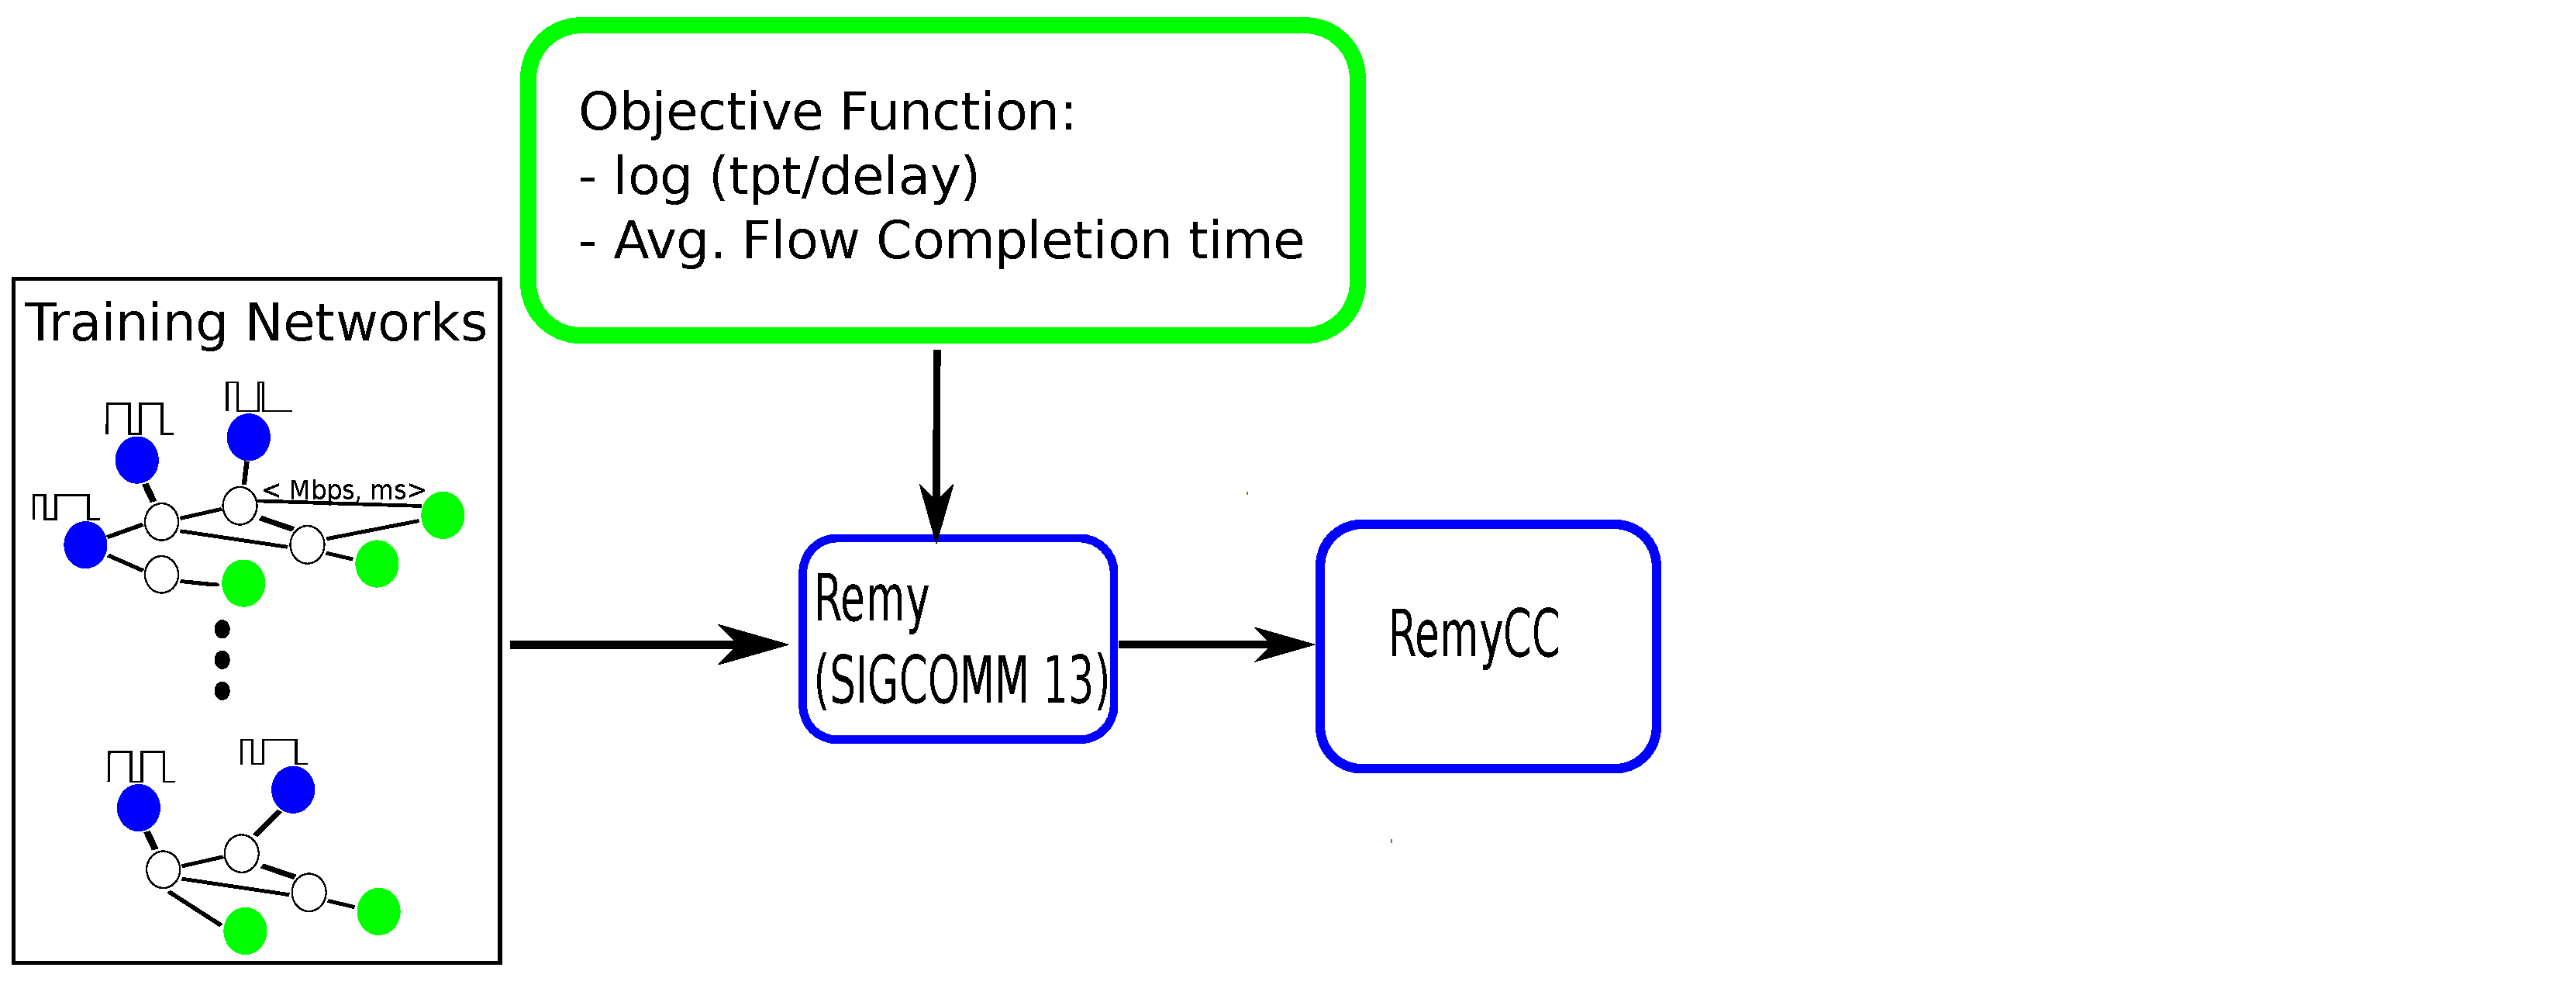
\includegraphics[width=3.5 in]{mechanize-4.pdf}}\only<5>{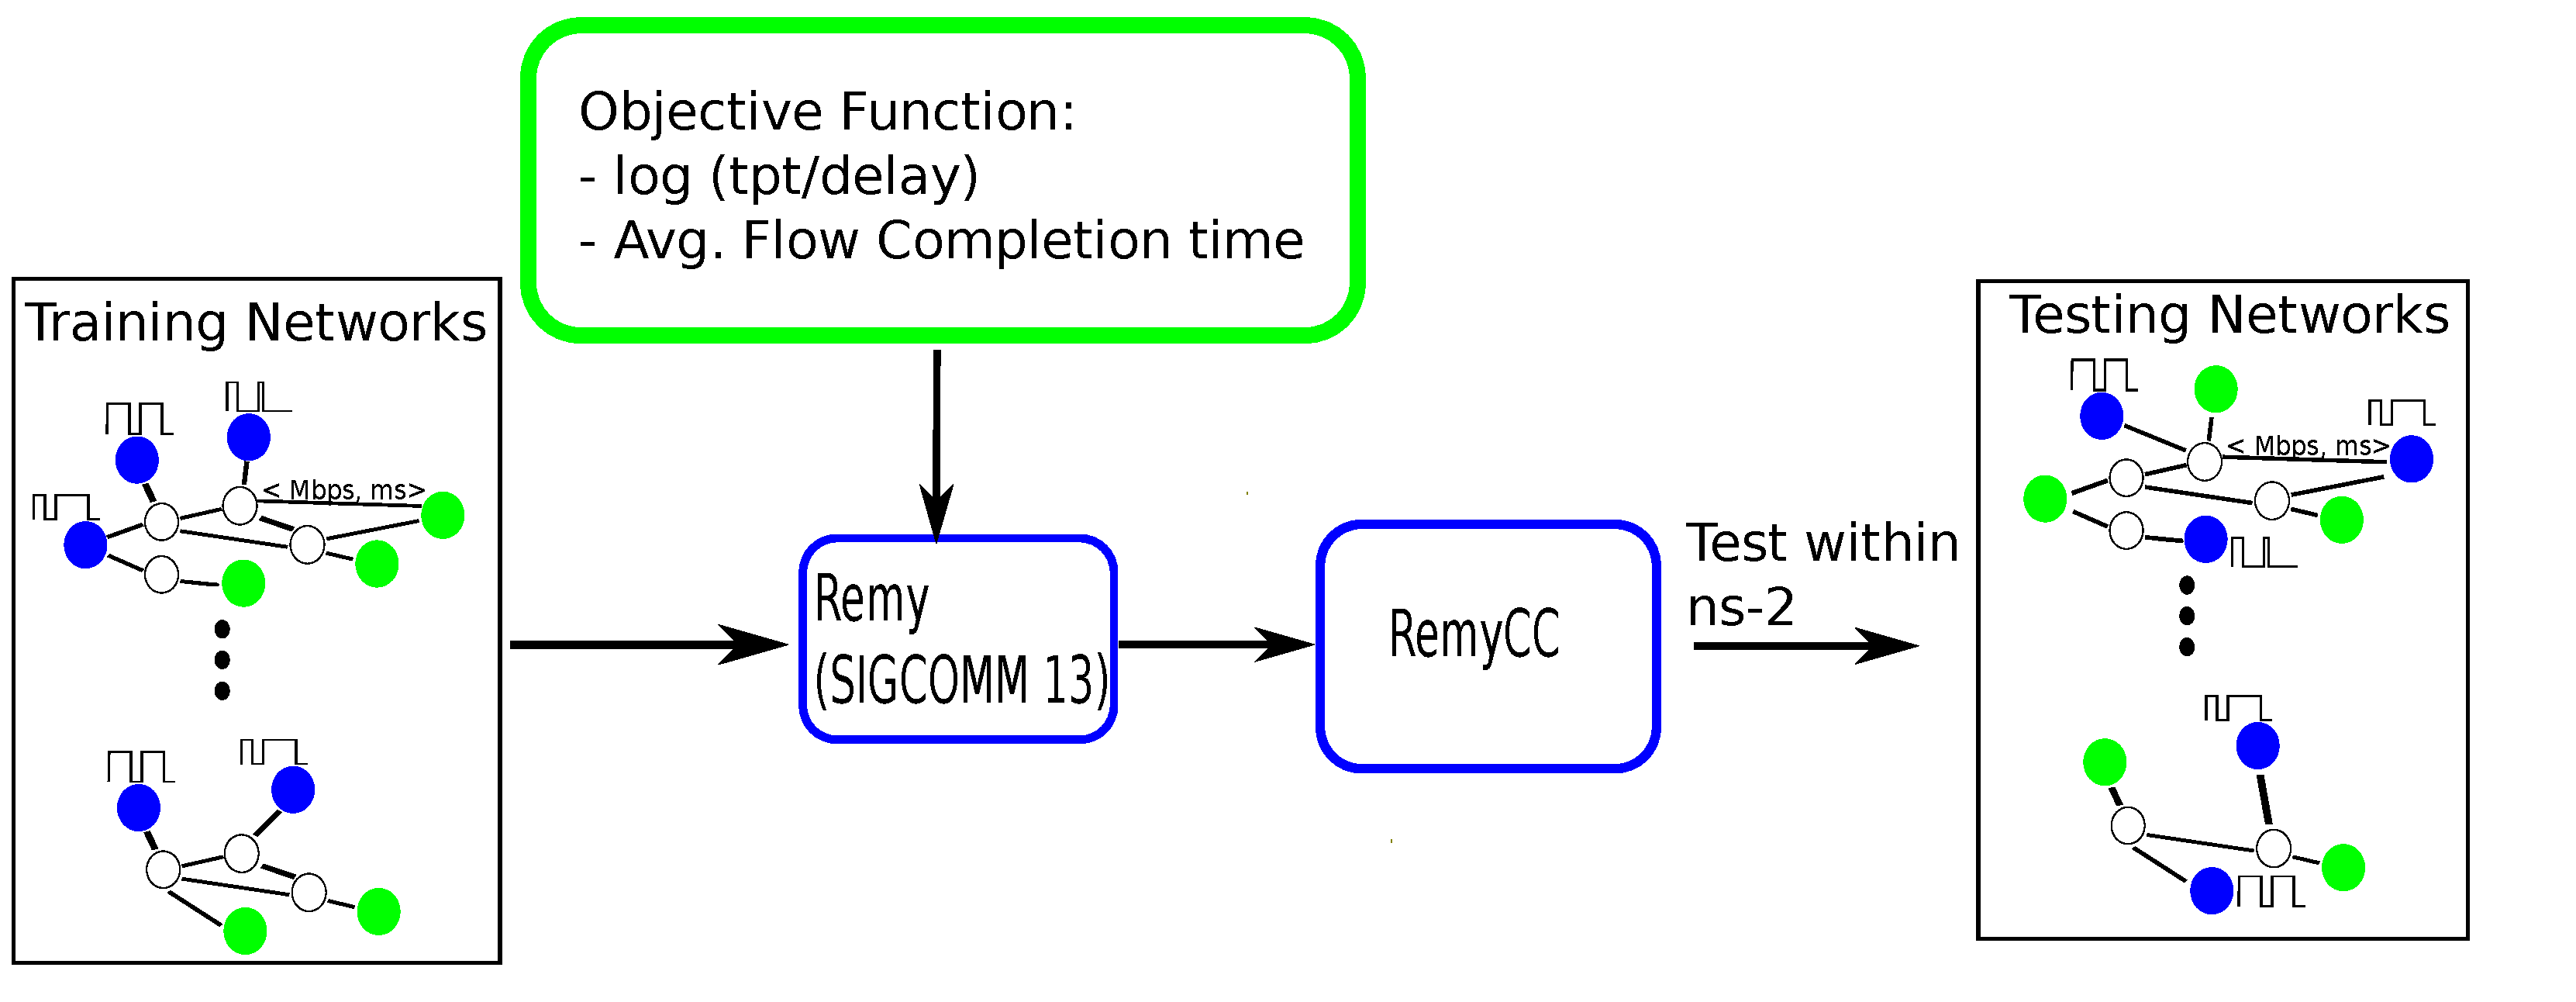
\includegraphics[width=3.5 in]{mechanize-5.pdf}}
\end{frame}

\input caveats

\begin{frame}
\frametitle{The learnability of congestion control}
\begin{itemize}
\item RemyCC compared with an omniscient protocol
\item Link speed
\item Degree of multiplexing
\item Topology
\item Knowledge of other senders
\end{itemize}
\end{frame}

\begin{frame}
\frametitle{The learnability of congestion control}
\begin{itemize}
\item \textcolor{blue}{RemyCC compared with an omniscient protocol}
\item \textcolor{gray}{Link speed}
\item \textcolor{gray}{Degree of multiplexing}
\item \textcolor{gray}{Topology}
\item \textcolor{gray}{Knowledge of other senders}
\end{itemize}
\end{frame}

\input optimality

\begin{frame}
\frametitle{The learnability of congestion control}
\begin{itemize}
\item \textcolor{gray}{RemyCC compared with an omniscient protocol}
\item \textcolor{blue}{Link speed}
\item \textcolor{gray}{Degree of multiplexing}
\item \textcolor{gray}{Topology}
\item \textcolor{gray}{Knowledge of other senders}
\end{itemize}
\end{frame}

\input linkspeed

\begin{frame}
\frametitle{The learnability of congestion control}
\begin{itemize}
\item \textcolor{gray}{RemyCC compared with an omniscient protocol}
\item \textcolor{gray}{Link speed}
\item \textcolor{blue}{Degree of multiplexing}
\item \textcolor{gray}{Topology}
\item \textcolor{gray}{Knowledge of other senders}
\end{itemize}
\end{frame}

\input multiplexing

\begin{frame}
\frametitle{The learnability of congestion control}
\begin{itemize}
\item \textcolor{gray}{RemyCC compared with an omniscient protocol}
\item \textcolor{gray}{Link speed}
\item \textcolor{gray}{Degree of multiplexing}
\item \textcolor{blue}{Topology}
\item \textcolor{gray}{Knowledge of other senders}
\end{itemize}
\end{frame}

\input topology 

\begin{frame}
\frametitle{The learnability of congestion control}
\begin{itemize}
\item \textcolor{gray}{RemyCC compared with an omniscient protocol}
\item \textcolor{gray}{Link speed}
\item \textcolor{gray}{Degree of multiplexing}
\item \textcolor{gray}{Topology}
\item \textcolor{blue}{Knowledge of other senders}
\end{itemize}
\end{frame}

\input compatibility

\begin{frame}
\frametitle{The learnability of congestion control}
\noindent
\begin{itemize}
\item<1-> \textcolor{green}{Possible to design for wide link speed range}
\item<2-> \textcolor{red}{Tension between low and high multiplexing}
\item<3-> \textcolor{green}{Simplifying topology may be acceptable}
\item<4-> \textcolor{red}{TCP compatibility is a double-edged sword}
\item<6-> Ongoing work in using findings to:
\begin{itemize}
\item<7-> improve Google's datacenter transport
\item<8-> user-space implementation of RemyCC
\end{itemize}
\item<9-> http://web.mit.edu/remy/learnability
\end{itemize}
\end{frame}

\end{Large}

\begin{frame}
\frametitle{Backup slides}
\end{frame}
\input caveats

\input remy


\input topology
\input diversity
\end{document}
